\section{Materialien}
\subsection{Hardware}
\subsubsection{Rechner 1} \todo {alle}
Noch nicht klar.XMG?
\subsubsection{Rechner 2} \todo {alle}
Noch nicht klar.
\subsubsection{HTC Vive} \todo {Laura}
Bei der HTC Vive handelt es sich um ein Head-Mounted Display, welches von HTC in Kooperation mit Valve \cite{website:Valve} produziert wird. Vorgestellt wurde dieses am 1. März 2015 im Vorfeld der Mobile World Congress \cite{website:mobileworldcongress}.\\
Die Auflösung des Displays beträgt insgesamt 2160x1200 Pixel, was 1080x1200 Pixeln pro Auge enstpricht. Die Brille bietet ein Sichtfeld von bis zu 110$^\circ$ bei einer Bildwiederholrate von 90 Hz \cite{website:HTC_Vive}. Zur Positionsbestimmung im Raum wird die Lighthousetechnologie von Valve genutzt. Zusätzlich sind neben einem Gyrosensor auch ein Beschleunigungsmesser und ein Laser-Positionsmesser verbaut. Mittels speziellen Game-Controllern wird eine Interaktion mit virtuellen Objekten ermöglicht. Die eingebaute Frontkamera wird für dieses Projekt nicht verwendet. Stattdessen wird auf die Ovrvision Pro zurückgegriffen, die im Folgenden in \ref{ovrvision} beschrieben wird.

\subsubsection{Ovrvision Pro \label{ovrvision}} \todo {Laura}
Bei der Ovrvision Pro handelt es sich um eine open-source Stereokamera, welche über USB 3.0 mit dem Rechner verbunden werden kann \cite{website:ovrvision}. Sie ist kompatibel mit Programmen wie Unity, welches für das Projekt benutzt wurde und in \ref{unity} beschrieben wird. 
\textcolor{red}{Nicht fertig. Brauchen wir das noch??}
1280x960x2	45fps	H115 V105



\subsubsection{Spielfeldkamera} \todo {Vera}
IDS uEye 164xLE

\subsubsection{Leap Motion} \todo {Laura}

\begin{figure}[H]
		\center 
		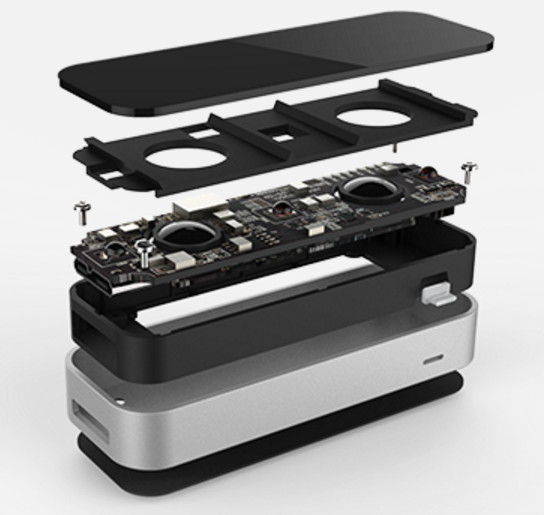
\includegraphics[width=6cm]{Bilder/leap-motion.png}
			\label{fig:leapMotion}
			\caption{Explosionszeichnung der Leap Motion. Quelle \cite{website:LeapMotionBlog}.}
	\end{figure}
	
Bei der Leap Motion \cite{website:LeapMotion} handelt sich um ein 7,6 x 3 x 1,3 cm großes Gerät, welches es mit Hilfe von Sensoren möglich macht, Hand- und Fingerbewegungen als Eingabemöglichkeit zu nutzen. Die Idee dahinter ist, eine Eingabegerät analog zu Maus zu schaffen, welches keinen direkten Kontakt bzw. keine Berührung benötigt. Hergestellt wird die Leap Motion von der Firma Leap Motion, Inc., die ihren Hauptsitz in Amerika hat. Gegründet wurde die Firma am 1. November 2010. \\
Wie auf Abbildung \ref{fig:leapMotion} erahnt werden kann, besteht das Gerät im wesentlich aus zwei integrierten weitwinkel Kameras und 3 einfachen Infrarot LEDs. Die LEDs haben jeweils eine Wellenlänge von 850 nm. Der durch die beiden Kameras aufgespannte Interaktionsraum der Leap Motion ähnelt einer umgedrehten Pyramide, mit einem Flächeninhalt von knapp 243 $cm{^2}$. \\
Für das Projekt wurde die Orion beta software, die in \ref{OBS} näher beschrieben wird. Diese Software ermöglicht unter anderem eine Erweiterung der Reichweite der Leap Motion von 60cm auf 80cm. Diese Reichweite ist durch die Ausbreitung der LED Lichter räumlich begrenzt. Die Lichtintensität der LEDs ist wiederum durch den maximalen Strom, der über die USB-Verbindung fließt beschränkt. \\


\subsection{Marker}\todo {Laura}
\subsubsection{ArUco Marker}\todo {Laura}
Da sowohl für die Marker, die für den eigentlichen Trackingalgorithmus verwendet werden, als auch für säntliche Marker, die zur Kalibrierung des Systems zum Einsatz kommen ArUco Marker verwendet werden, werden diese im Folgenden kurz erläutert.\\
ArUco Marker bestehen ähnlich wie QR-Codes aus einer zweidimensionalen Matrix, aus schwarzen und weißen Quadraten, die die kodierten Daten binär darstellen. Die ArUco Bibliothek kann für Augmented Reality Anwendungen genutzt werden und basiert ausschließlich auf der OpenCV Bibliothek. 
 
\subsubsection{Trackingmarker}\todo {Laura}
Das System umfasst 12 Marker über die das Tracking realisiert wird. Alle Marker stimmen in Form und Farbe, sowie Material und Oberflächenbeschaffenheit überein. Sie sind würfelförmig und haben eine Kantenlänge von 46mm. Die Kanten sind in einem Winkel von 45$^\circ$ angefast. Die Marker bestehen aus Aluminium, welches glasperlgestrahlt ist um eine matte Oberfläche zu erzeugen. Auf die Oberseite des Markers ist mittig ein grünes Quadrat mit einer Kantenlänge von 40mm aufgebracht. Auf diesem ist, ebenfalls mittig, ein 35 mm großer ARUCO-Marker, welcher aus dem $\textit{DICT \_4X4 \_50}$ generiert wurde und einen Rand von einem bit hat. Jeder Marker hat einen einzigartigen ARUCO-Marker, der einer Id von 1-12 entspricht. 


	\begin{figure}[H]
		\center 
		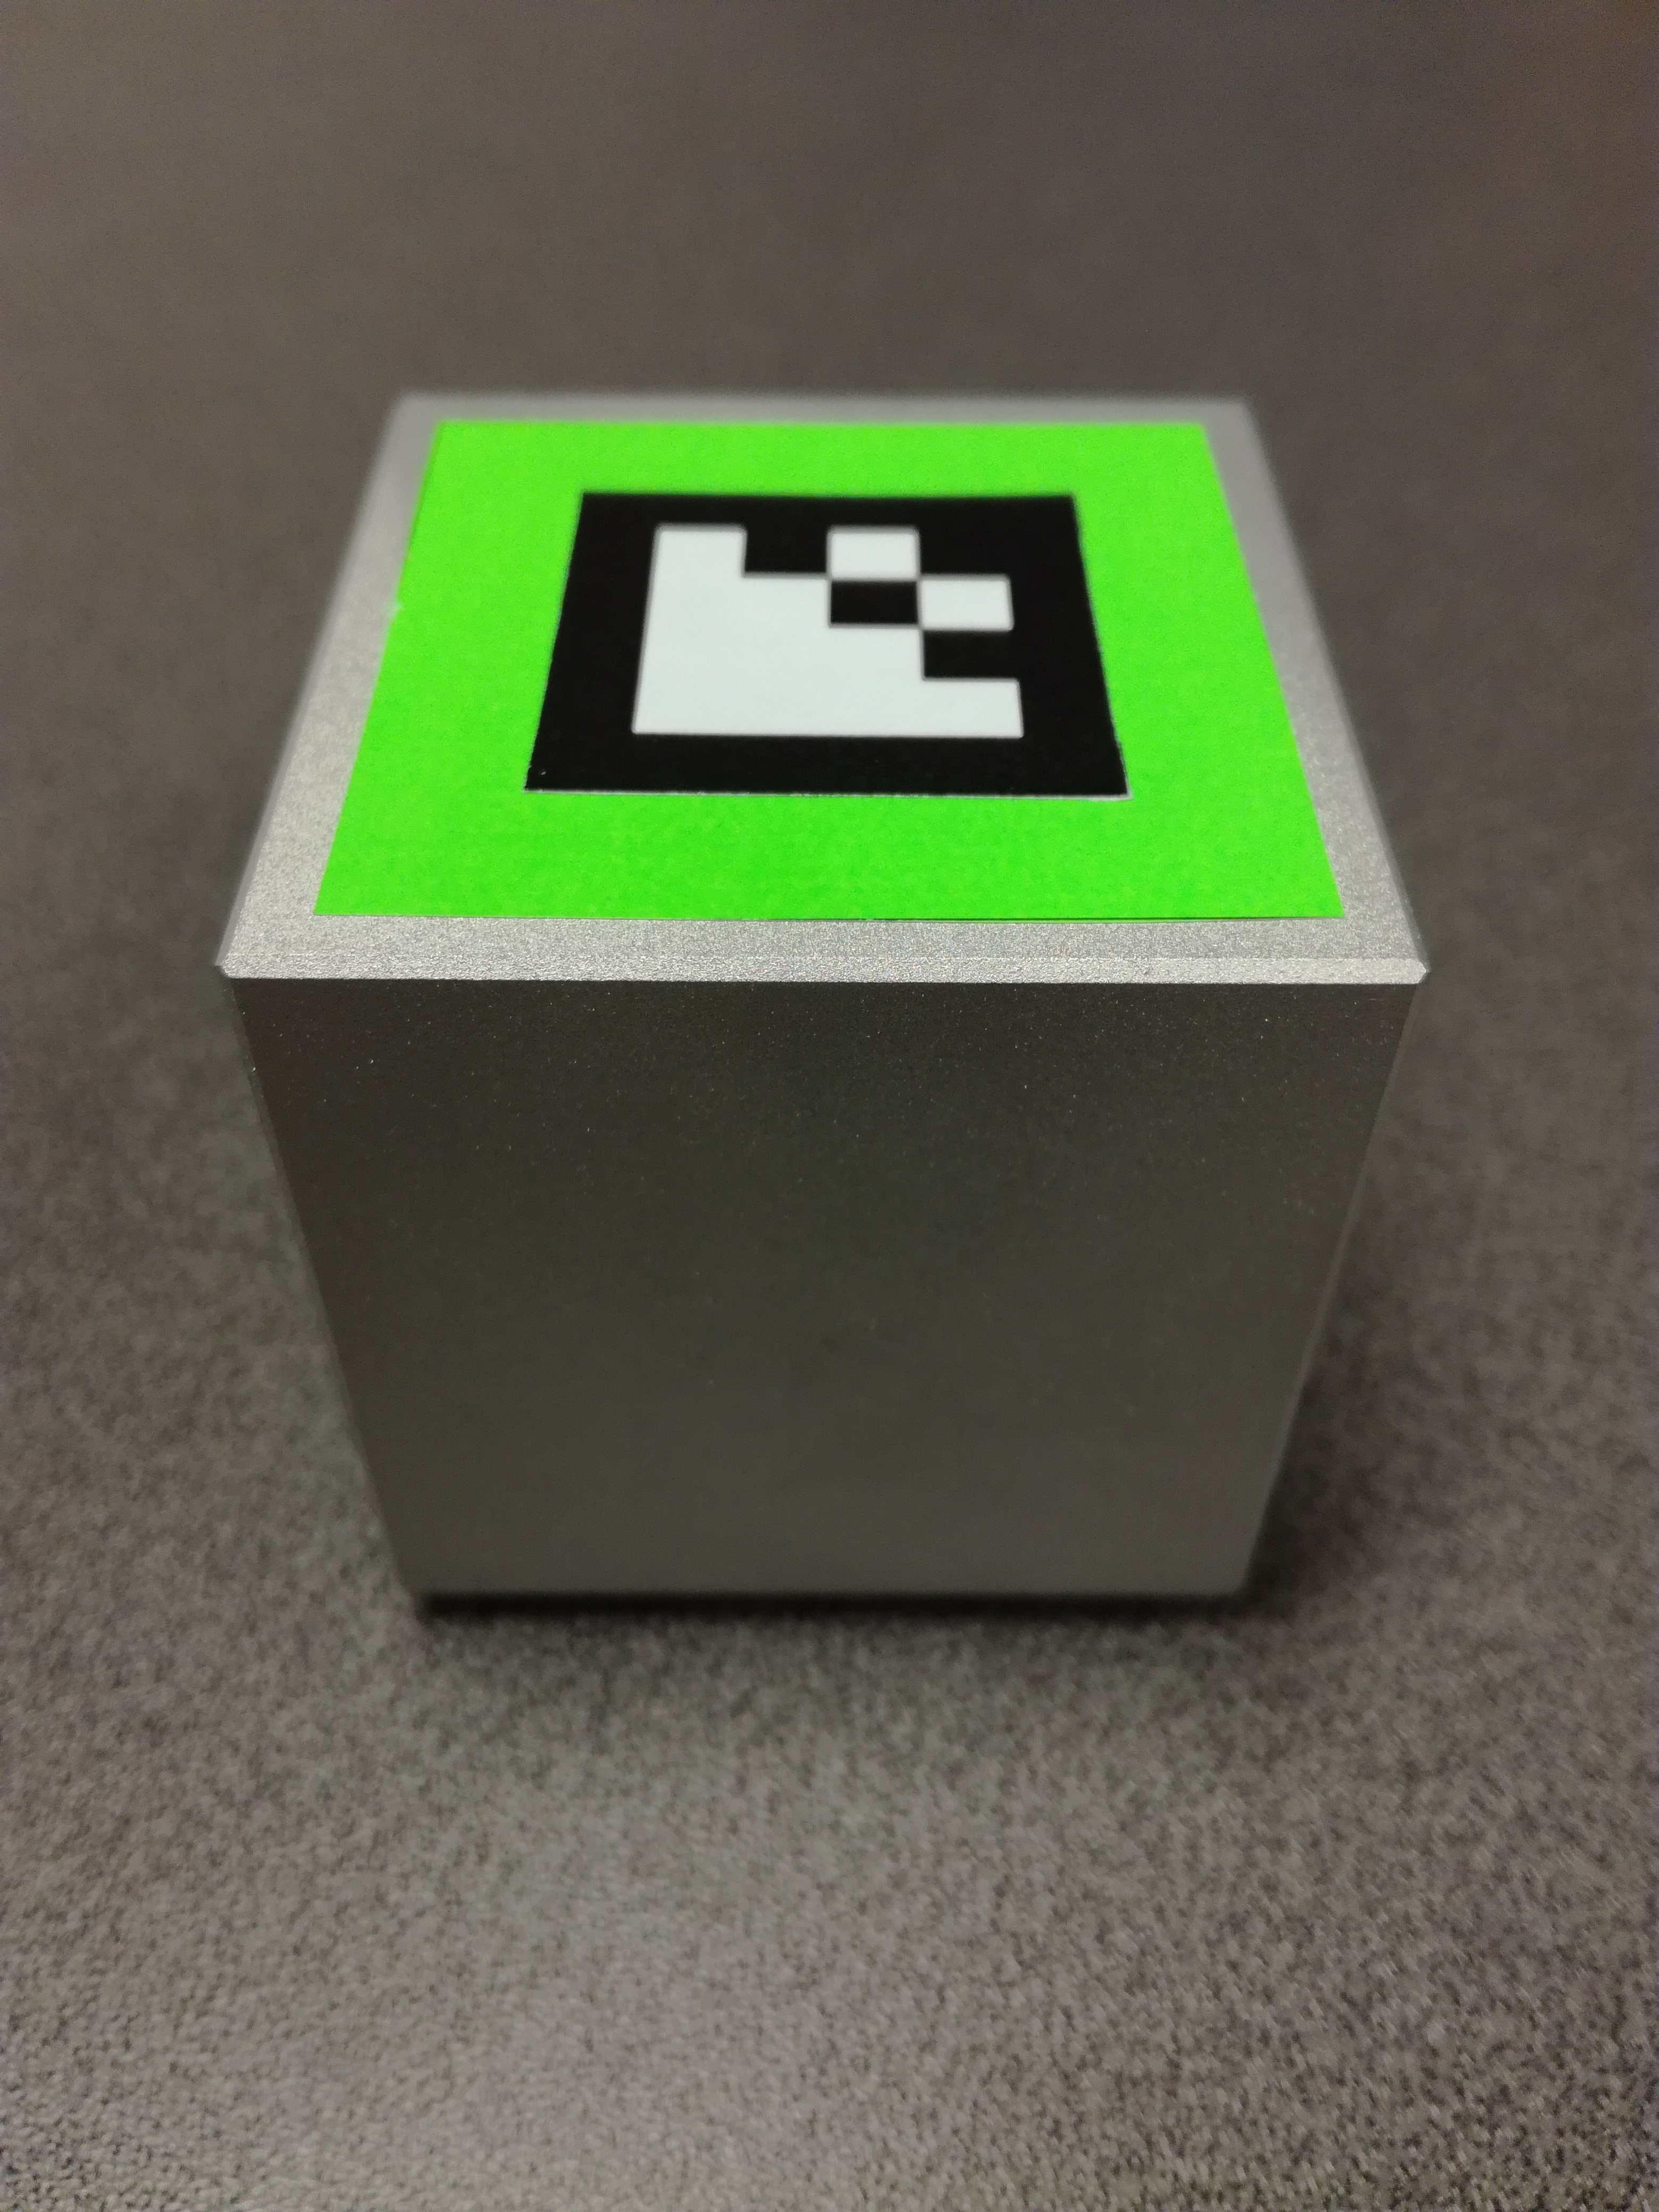
\includegraphics[trim = 0mm 280mm 0mm 150mm, clip, width=6cm]{Bilder/tracking-marker.jpg}
			\label{fig:marker}
			\caption{Trackingmarker mit der ID \textcolor{red}{??}.}
	\end{figure}


\subsubsection{Spielfeldkalibrierung}\todo {Lukas}
Marker auf schwarzen Holzplatten von Luke

\subsubsection{Marker uEye Kalibrierung}\todo {Vera}
Poster von Vera

\subsection{Software}
\subsubsection{Unity \label{unity}} \todo {Paul oder Lukas}
\subsubsection{Visual Studio} \todo {Laura}
\subsubsection{OpenCV} \todo {Vera}
Wo führen wir die dlls auf die du erzeugt hast??
\subsubsection{Ovrvision Pro SDK} \todo {Paul oder Lukas}
\subsubsection{Leap Motion SDK} \todo {Laura}
\textcolor{red}{
Once the image data is streamed to your computer, it’s time for some heavy mathematical lifting. Despite popular misconceptions, the Leap Motion Controller doesn’t generate a depth map – instead it applies advanced algorithms to the raw sensor data.}

The Leap Motion Service is the software on your computer that processes the images. After compensating for background objects (such as heads) and ambient environmental lighting, the images are analyzed to reconstruct a 3D representation of what the device sees.

Next, the tracking layer matches the data to extract tracking information such as fingers and tools. Our tracking algorithms interpret the 3D data and infer the positions of occluded objects. Filtering techniques are applied to ensure smooth temporal coherence of the data. The Leap Motion Service then feeds the results – expressed as a series of frames, or snapshots, containing all of the tracking data – into a transport protocol.

Through this protocol, the service communicates with the Leap Motion Control Panel, as well as native and web client libraries, through a local socket connection (TCP for native, WebSocket for web). The client library organizes the data into an object-oriented API structure, manages frame history, and provides helper functions and classes.

From there, the application logic ties into the Leap Motion input, allowing a motion-controlled interactive experience. Next week, we’ll take a closer look at our SDK and getting started with our API. \cite{website:LeapMotionBlog}

\subsubsection{Orion Beta Software} \label{OBS}

\subsubsection{uEye SDK}\todo {Vera}
\subsubsection{Steam VR}\todo {Paul oder Lukas}


\newpage